\chapter{Executive summary (read this first)}

\section{What the two projects are, in one paragraph each}
\textbf{VAE-Triage (pathology).} A whole-slide image (WSI) of an H\&E-stained breast lymph-node section is a
$\sim$100{,}000 $\times$ 200{,}000-pixel pyramidal TIFF. Most of it is empty glass, and some tissue tiles are
unusable (out of focus, pen ink, folds, bubbles). Running a heavy segmentation network on every tile wastes
GPU time and produces garbage on artefacts. VAE-Triage is a \emph{gate in front of the heavy model}:
it tiles the slide lazily, throws away glass, flags bad tiles and keeps a compact description of the good
tiles. In this study we rebuilt it as an \textbf{edge-first, Gaussian-Mixture-Model (GMM) pipeline} that runs
on a CPU next to the scanner, and we kept the original VQ-VAE as an optional deep component.

\textbf{Satellite\_based\_tile\_segmentation (segmentation).} Semantic segmentation of 6000$\times$6000-pixel
aerial orthophotos (ISPRS Potsdam, 6 classes) with a residual U-Net with a dilated (ASPP-like) bottleneck,
patch-based training, overlap stitching and 8$\times$ test-time augmentation. The \emph{engineering problem is
identical to WSI segmentation}: an image too large for the network is cut into patches, predicted, and stitched
back. This is the project to talk about when the interviewer asks ``how do you do segmentation?''.

\section{Pipeline at a glance}
\begin{figure}[H]\centering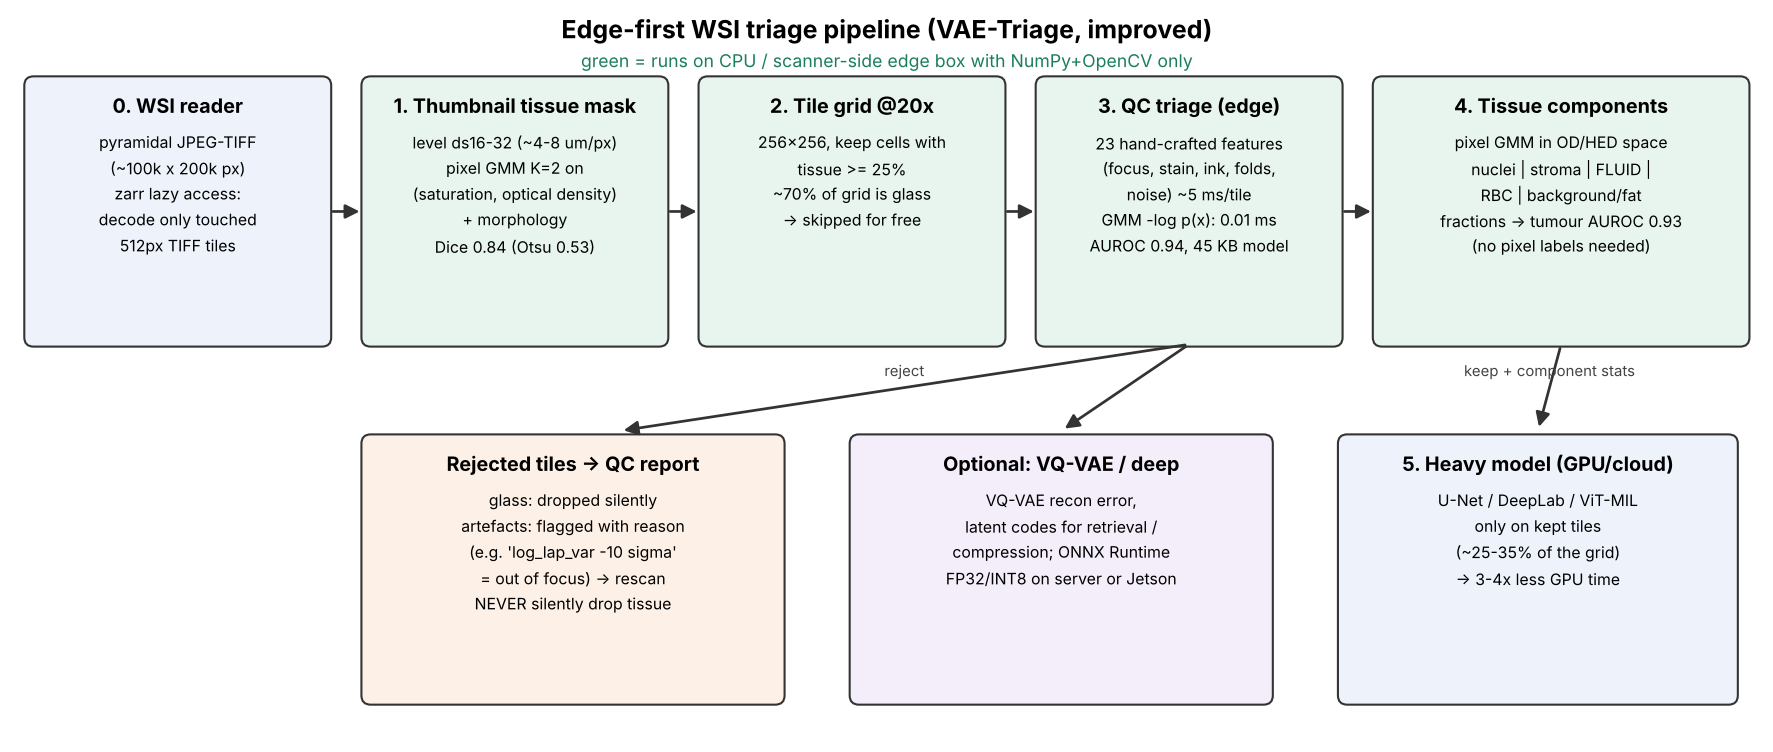
\includegraphics[width=\linewidth]{pipeline_pathology.png}
\caption{The improved VAE-Triage pipeline. Everything in green runs on a CPU with NumPy + OpenCV only.}\end{figure}

\section{Headline numbers (all measured in this study)}
Data: 7 real CAMELYON16 breast lymph-node WSIs (4.5\,GB, 203{,}168 tiles at 20$\times$), expert tumour masks;
ISPRS Potsdam RGB+NIR, 6 training tiles + 3 official test tiles. CPU only (4 vCPU), no GPU.

\begin{table}[H]\centering\small
\begin{tabular}{p{5.3cm}p{5.2cm}p{5.4cm}}\toprule
\textbf{Task} & \textbf{Best classical / ours} & \textbf{Reference points}\\\midrule
Stage 0: tissue vs glass (Dice) & \textbf{GMM K=2 on (S, OD): 0.839} & Otsu 0.52--0.55; fixed thr.\ 0.74; k-means 0.14\\
Compute removed before any NN & \textbf{69.6\% of 203k tiles are glass} & 30--78\% per slide\\
Stage 1: tile QC (AUROC / F1) & \textbf{GMM 0.939 / 0.897}, single Gaussian 0.954 / 0.906 & Laplacian 0.76; HistoQC-style rules 0.86; IsolationForest 0.91; supervised LR/RF 0.96--0.97\\
Tumour wrongly rejected by QC & \textbf{3.5\%} with slide-level calibration & 43\% with naive same-slide calibration (a trap!)\\
Original VQ-VAE MSE as QC score & AUROC \textbf{0.376} (worse than chance) & blur/glass reconstruct \emph{better} than tissue\\
Supervised MobileNetV3 QC & AUROC 0.976, 0.6\,ms/tile (ORT) & but recall 7--64\% on artefact types not in training; GMM 64--99\%\\
QC model size / cost & \textbf{45\,KB JSON, 1{,}799 numbers, 0.01\,ms/tile} + 2.1\,ms features (128\,px) & VQ-VAE 0.69\,M params, 22.9\,ms/tile ORT\\
Tumour vs normal, no tumour labels & GMM novelty 0.740; VQ-VAE 0.749 & Lit.\ plain AE 0.66, L1-AE 0.21, perceptual AE 0.93\\
Tumour via GMM tissue components (fluid, nuclei, stroma) & \textbf{0.931} (5 numbers per tile + LR) & supervised RF on 23 features 0.945\\
Potsdam segmentation (mIoU, 5 cls) & repo U-Net, 30\,min CPU: \textbf{58.2} (8$\times$TTA \textbf{61.3}); GMM-Bayes + smoothing 48.5; RF+NIR 50.4 & k-means 19.8; lit.\ deep SOTA (GPU) 86.5--87.5\\
Car instance segmentation (Potsdam) & YOLOv8n-seg, 20\,min CPU: \textbf{car IoU 84.7}, mask mAP50 0.85 & U-Net car IoU 61; RF 46\\
\bottomrule\end{tabular}\caption{Summary. Deep-learning rows and the time-boxed U-Net / YOLO runs are in the
chapters and in the auto-generated tables.}\end{table}

\section{The six things the candidate must be able to say}
\begin{enumerate}
\item \textbf{Why triage at all:} 70\% of a slide is glass and a few \% is unusable; the GPU model should only see the
remaining $\sim$30\%. That is a 3--4$\times$ saving before any clever model.
\item \textbf{Why a GMM and not a deep net for this gate:} the decision ``is this tile normal-looking'' is a
\emph{density estimation} problem; a GMM on 23 physically meaningful features gives 0.94 AUROC with a 45\,KB model,
microsecond scoring, no GPU, no labels, and a human-readable reason for every rejection.
\item \textbf{Why a GMM and not k-means or Otsu:} k-means is a GMM with equal spherical covariances and hard
assignments, so it splits large elongated clusters (stroma, fluid) and merges small ones; Otsu assumes one
threshold on one channel. Measured: GMM Dice 0.84 vs Otsu 0.53 vs k-means 0.14 for tissue; only the GMM separates
a fluid component.
\item \textbf{The calibration trap:} if the reject threshold is set on tiles from the same slides it was fitted on,
43\% of tumour tiles are rejected on new slides. Calibrate on \emph{unseen slides} (leave-one-slide-out) -- 3.5\%.
\item \textbf{The VQ-VAE finding:} reconstruction error ranks blurred and empty tiles as \emph{more} normal (AUROC 0.38),
so it must not be the QC score; keep the VQ-VAE as a compressor/tokeniser and a tumour-novelty signal (0.75).
\item \textbf{Where deep learning is still needed:} the actual diagnosis (tumour segmentation, grading) -- that is
the U-Net project. Supervised deep models beat everything when labels exist; the GMM gate decides \emph{where} to
spend that compute.
\end{enumerate}

\warn{Do not claim numbers that are not in this report. The original README of the satellite repo lists per-class
IoUs (e.g.\ building 0.85, car 0.82) that are not reproduced by any script in the repository. Say ``on our
re-run we get X''. Also: the original VAE-Triage training script crashed (Section~\ref{sec:bugs}); be honest that
it was fixed during preparation.}
